%%%%%%%%%%%%%%%%%%%%%%%%%%%%%%%%%%%%%%%%%%%%%%%%%%%%%%%%%%%%%%%%%%%%%%%%%%%%%%%%
%%%%%%%%%%%%%%%%%%   Vorlage für eine Abschlussarbeit   %%%%%%%%%%%%%%%%%%%%%%%%
%%%%%%%%%%%%%%%%%%%%%%%%%%%%%%%%%%%%%%%%%%%%%%%%%%%%%%%%%%%%%%%%%%%%%%%%%%%%%%%%

% Erstellt von Maximilian Nöthe, <maximilian.noethe@tu-dortmund.de>
% ausgelegt für lualatex und Biblatex mit biber

% Kompilieren mit
% latexmk --lualatex --output-directory=build thesis.tex
% oder einfach mit:
% make

\documentclass[
  tucolor,       % remove for less green,
  BCOR=12mm,     % 12mm binding corrections, adjust to fit your binding
  parskip=half,  % new paragraphs start with half line vertical space
  open=any,      % chapters start on both odd and even pages
  cleardoublepage=plain,  % no header/footer on blank pages
]{tudothesis}


% Warning, if another latex run is needed
\usepackage[aux]{rerunfilecheck}

% just list chapters and sections in the toc, not subsections or smaller
\setcounter{tocdepth}{1}

%------------------------------------------------------------------------------
%------------------------------ Fonts, Unicode, Language ----------------------
%------------------------------------------------------------------------------
\usepackage{fontspec}
\defaultfontfeatures{Ligatures=TeX}  % -- becomes en-dash etc.

% load english (for abstract) and ngerman language
% the main language has to come last
\usepackage[american, ngerman]{babel}

% intelligent quotation marks, language and nesting sensitive
\usepackage[autostyle]{csquotes}

% microtypographical features, makes the text look nicer on the small scale
\usepackage{microtype}

%------------------------------------------------------------------------------
%------------------------ Math Packages and settings --------------------------
%------------------------------------------------------------------------------

\usepackage{amsmath}
\usepackage{amssymb}
\usepackage{mathtools}

% Enable Unicode-Math and follow the ISO-Standards for typesetting math
\usepackage[
  math-style=ISO,
  bold-style=ISO,
  sans-style=italic,
  nabla=upright,
  partial=upright,
  warnings-off={mathtools-colon,mathtools-overbracket}, % suppress some unnecessary warnings
]{unicode-math}
\setmathfont{Latin Modern Math}

% nice, small fracs for the text with \sfrac{}{}
\usepackage{xfrac}


%------------------------------------------------------------------------------
%---------------------------- Numbers and Units -------------------------------
%------------------------------------------------------------------------------

\usepackage[
  locale=DE,
  separate-uncertainty=true,
  per-mode=symbol-or-fraction,
]{siunitx}

%------------------------------------------------------------------------------
%-------------------------------- tables  -------------------------------------
%------------------------------------------------------------------------------

\usepackage{booktabs}       % \toprule, \midrule, \bottomrule, etc

%------------------------------------------------------------------------------
%-------------------------------- graphics -------------------------------------
%------------------------------------------------------------------------------

\usepackage{graphicx}
% currently broken
% \usepackage{grffile}

% allow figures to be placed in the running text by default:
\usepackage{scrhack}
\usepackage{float}
\floatplacement{figure}{htbp}
\floatplacement{table}{htbp}

% keep figures and tables in the section
\usepackage[section, below]{placeins}

% allows to include PDFs as full pages
\usepackage{pdfpages}

% Set the PDF Version of this document to 1.7 (1.4 is the current default)
% This is needed so that PDFs with Version >1.5 can be included
\pdfvariable minorversion=7

%------------------------------------------------------------------------------
%---------------------- customize list environments ---------------------------
%------------------------------------------------------------------------------

\usepackage{enumitem}

%------------------------------------------------------------------------------
%------------------------------ Bibliographie ---------------------------------
%------------------------------------------------------------------------------

\usepackage[
  backend=biber,   % use modern biber backend
  autolang=hyphen, % load hyphenation rules for if language of bibentry is not
                   % german, has to be loaded with \setotherlanguages
                   % in the references.bib use langid={en} for english sources
]{biblatex}
\addbibresource{references.bib}  % the bib file to use
\DefineBibliographyStrings{german}{andothers = {{et\,al\adddot}}}  % replace u.a. with et al.


% Last packages, do not change order or insert new packages after these ones
\usepackage[pdfusetitle, unicode, linkbordercolor=tugreen, citebordercolor=tugreen]{hyperref}
\usepackage{bookmark}
\usepackage[shortcuts]{extdash}

%------------------------------------------------------------------------------
%-------------------------    Angaben zur Arbeit   ----------------------------
%------------------------------------------------------------------------------

\author{Sebastian Fischer}
\title{\LaTeX-Dokumentenklasse und Vorlage für Abschlussarbeiten an der TU Dortmund}
\date{2025}
\birthplace{Göttingen}
\chair{Arbeitsgruppe Astroteilchenphysik}
\division{Fakultät Physik}
\thesisclass{Bachelor of Science}
\submissiondate{11.01.2025}
\firstcorrector{Prof.~Dr.~Dr. Wolfgang Rhode}
\secondcorrector{Prof.~Dr.~Zweitgutachter}

% tu logo on top of the titlepage
\titlehead{\includegraphics[height=1.5cm]{logos/tu-logo.pdf}}

\begin{document}
\frontmatter
% \thispagestyle{empty}
% \setcounter{page}{2}
% \section*{Hinweise}
% Empfohlen wird die Verwendung dieser Vorlage mit der jeweils aktuellsten TeXLive Version (Linux, Windows) bzw. MacTeX Version (MacOS).
% Aktuell ist dies TeXLive 2021. Download hier:
% \begin{center}
%   \ttfamily\url{https://www.tug.org/texlive/}
% \end{center}

% Die Vorlage \texttt{thesis.tex} ist für die Kompilierung mit \texttt{lualatex} ausgelegt, mit wenigen Anpassungen kann sie aber auch mit \texttt{pdflatex} oder \texttt{xelatex} verwendet werden.
% Die Dokumentenklasse \texttt{tudothesis.cls} kann mit allen drei Programmen verwednet werden.

% Achten Sie auch auf die Kodierung der Quelldateien.
% Bei Verwendung von Xe\LaTeX\ oder Lua\LaTeX\ (empfohlen) müssen die
% Quelldateien UTF-8 kodiert sein.
% Bei Verwendung von pdf\LaTeX\ nutzen Sie die Pakete \texttt{inputenc} und \texttt{fontenc} mit der korrekten Wahl der Kodierungen.

% Eine aktuelle Version dieser Vorlage steht unter 
% \begin{center}
%   \ttfamily\url{https://github.com/maxnoe/tudothesis}
% \end{center}
% zur Verfügung.

% Alle verwendeten Pakete werden im \LaTeX{} Kurs von Pep et al.\ erklärt:
% \begin{center}
%   \ttfamily\url{http://toolbox.pep-dortmund.org/notes}
% \end{center}

% Für Rückmeldungen und bei Problemen mit der Klasse oder Vorlage, bitte ein \emph{Issue} auf GitHub aufmachen oder eine Email an
% \href{mailto:maximilian.noethe@tu-dortmund.de}{maximilian.noethe@tu-dortmund.de} schreiben.

% Wenn Sie die Dokumentenklasse mit der Option \texttt{tucolor} laden, werden verschiedene Elemente in TU-Grün gesetzt.

\maketitle

% Gutachterseite
\makecorrectorpage

% hier beginnt der Vorspann, nummeriert in römischen Zahlen
% \thispagestyle{plain}

% \section*{Kurzfassung}
% Hier steht eine Kurzfassung der Arbeit in deutscher Sprache inklusive der Zusammenfassung der
% Ergebnisse.
% Zusammen mit der englischen Zusammenfassung muss sie auf diese Seite passen.

% \section*{Abstract}
% \begin{foreignlanguage}{english}
% The abstract is a short summary of the thesis in English, together with the German summary it has to fit on this page.
% \end{foreignlanguage}

\tableofcontents

\mainmatter
% Hier beginnt der Inhalt mit Seite 1 in arabischen Ziffern
\chapter{Einleitung}
% Hier folgt eine kurze Einleitung in die Thematik der Bachelorarbeit.
% Die Einleitung muss kurz sein, damit die vorgegebene Gesamtlänge der 
% Arbeit von 25 Seiten nicht überschritten wird. 
% Die Beschränkung der Seitenzahl sollte man ernst nehmen,
% da Überschreitung zu Abzügen in der Note führen kann. 
% Um der Längenbeschränkung zu genügen, darf auch nicht an der Schriftgröße,
% dem Zeilenabstand oder dem Satzspiegel (bedruckte Fläche der Seite) manipuliert werden.


The IceCube neutrino detector is a cubic kilometer scale particle detector located near the Amundsen-Scott South Pole Station. The primary goal of 
the detector is the detection of high energy neutrinos as messenger particles for study of astrophysical sources. The detector unit is split into three 
parts, which are the In-Ice Array, the IceTop, and the DeepCore. 

The In-Ice Array is the largest component and consists of 86 vertical strings, extending vertically into the ice below the surface for \SI{2450}{\metre}. 
Each of the strings contains 60 Digital Optical Modules (DOMs) starting from a depth of \SI{1450}{\metre} all the way down to \SI{2450}{\metre}
The DOMs are evenly separated by \SI{17}{\metre} alongside their respective string, making a total number of \num{5160} DOMs. 

The IceTop, as the name suggests, is located at the surface of the ice with \num{162} tanks filled with ice and equipped with PMTs. 
The tanks are arranged in 81 stations in a manner that approximately mimics the structure of the In-Ice Array. 

The DeepCore is a sub-array within the In-Ice Array and is located at depths beneath \SI{1750}{\metre}. It contains an extra \num{8} strings alongside the 
\num{7} strings from the In-Ice Array. This creates a more densly packed arrangement of DOMs in the lower center of the detector, which increases its 
ability to detect low-energy signals.

Figure~\ref{fig:icecube_sketch_01} shows a visual representation of this structure.

\begin{figure}[htbp]
    \centering
    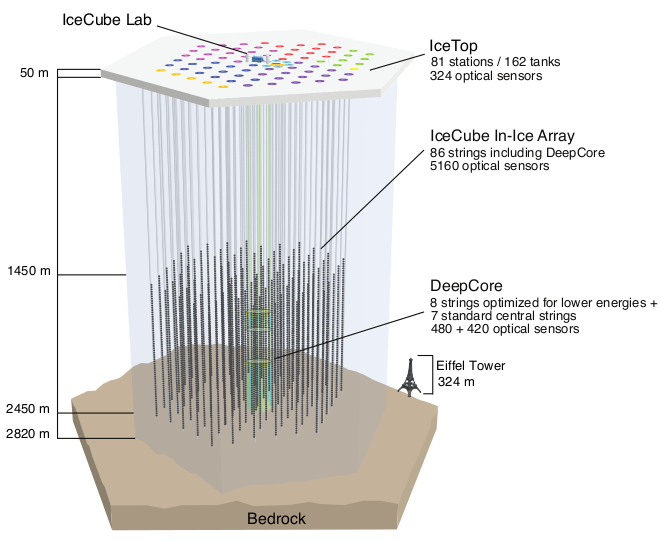
\includegraphics[width=\textwidth]{content/pictures/icecube_sketch_01.png}
    \caption{An overview of the arrangement inside of the detector.}\label{fig:icecube_sketch_01}
\end{figure}

\section{Digital Optical Module}

A single DOM consists of a glass housing, in which the PMT and the corresponding curcuit boards are located. The technical part of the functionality of 
the circuit boards are not of interest for this analysis, so I will not go into detail on that topic. The PMT however is the actual detecting unit of 
the DOM\. A sketch of a PMT is shown in figure~\ref{fig:pmt01}.

\begin{figure}[htbp]
    \centering
    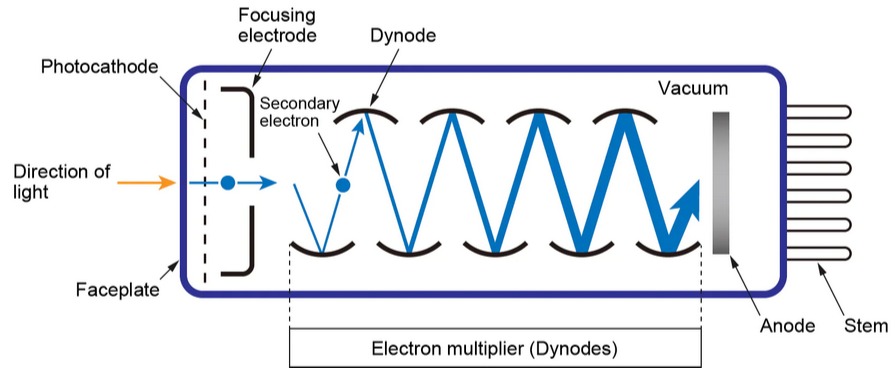
\includegraphics[width=\textwidth]{content/pictures/pmt_sketch_01.png}
    \caption{The principle construction of a photomultiplier.}\label{fig:pmt01}
\end{figure}

When a photon with sufficient energy hits the photocathode of the PMT, its energy gets absorbed and an electron is emitted via the photoelectric effect.
the electron is accelerated towards the first dynode due to its electric charge. Hitting the dynode triggers secondary emittions, increasing the total 
number of electrons emitted. This process repeats itself for however many dynodes are the PMT accompasses. After the final amplification by the last 
dynode the electrons are collected by the anode, which produces a current proportional to the intensity of the initial light signal, meaning the amount of
photons hitting the PMT\@. 

\section{Cherenkov radiation}

The light detected by the photomultipliers is only a secondary signal called Cherenkov radiation. It is created when a charged particle travels through a 
dielectric medium with a velocity greater than the speed of light inside of the medium. The charged particle polarizes the medium's molecules in its
immediate surroundings while passing through it. The excited molecules then return to their ground state by emitting their superfluous energy as light.
Because the light travels slower than the particle exciting the molecules, the light waves do not interfere destructively, but build a conical shock front 
similar in principle to that of an object, moving through air at supersonic velocities. This cone of light is the Cherenkov radiation detected by the PMTs.

\section{Muons}

A significant percentile of the particles measured in IceCube are muons, which are elementary particles categorized as leptons by the standard model.
This means they carry an electric charge of $\pm 1e$ and have spin $\frac{1}{2}$. The mass of the muon is \num{105.658}\text{MeV}. IceCube detects
muons at a rate of roughly \SI{2500}{Hz}. While they are muons originating from outer space that hit the earths surface, the vast majority of muons detected
on earth are created in the atmosphere. When cosmic rays collide with the atmosphere's molecules, a multitude of secondary particles are created including 
pions and kaons. The average lifetime of these mesons are of the magnitude of \SI{e8}{s} or less. Their resulting decay products include muons which are 
produced via the following decay modes:\\

\begin{align}
    \pi^\pm \to \mu^\pm + \nu_\mu \\
    K^\pm \to \mu^\pm + \nu_\mu
\end{align}

These muons have an average lifetime of about \SI{2.2}{ms}, which is enough for a significant amount of them reaching the earths surface due the their 
ultrarelativistic velocities. When a muon travels through the ice within IceCube, it produces Cherenkov radiation due to its charge and high velocities and 
can thus be indirectly measured.

\section{Data aquisition}\label{sec:daq}

A single DOM measureing a signal is not able to distinguish between different types of events, since its only capability lies in the detection of a current
caused by photons hitting the PMT\@. In order to distinguish between noise and possible signals stemming from Cherenkov radiation, multiple requirements are
put in place to ensure that the full data of a signal is only saved for those signals that might constitute a real event. The data aquisition systems (DAQ)
is the software complex responsible for filtering signals by different characteristics. The first step for any signal is to scan for so called hard local 
coincidences (HLC). 
There are so called triggers implemented which search for multiplicities of HLC hits within a certain time frame and with certain spatial requirements.
The simplest one is the simple multiplicity trigger (SMT), which triggers whenever at least $N$ HLC hits occur within a time frame of some 
\si{\micro\second}. This sets a set of intuitive conditions for grouping a cluster of signals into an event that could be a muon or another 
charged particle emitting Cherenkov radiation. 
Another trigger is the fixed rate trigger (FRT) which is of great importance for the analysis of this thesis. The FRT does not get triggered 
by any multiplicity of events. It is a timed trigger which reads out the entire detector, meaning all functioning DOMs for \SI{10}{ms}
every \SI{300}{s}. Since there are no conditions of any kind in place for this trigger, it saves everything being measured during the 
readout time frame. This allows a precise look into the low energy spectrum of signals hitting the detector which is significant for the 
analysis of the backround noise in IceCube. An overview of different triggers, which are not primarily significant for this thesis is shown 
in figure~\ref{fig:triggers}.

\begin{figure}[htbp]
    \centering
    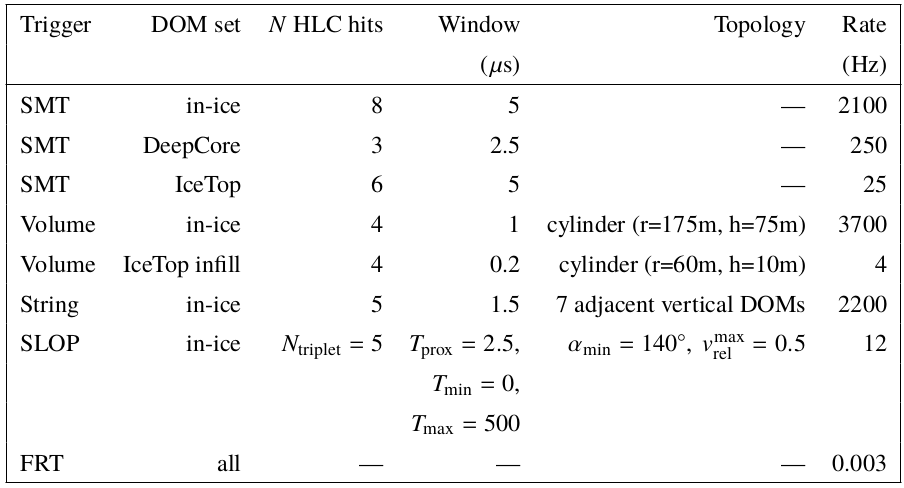
\includegraphics[width=\textwidth]{content/pictures/trigger_list.png}
    \caption{A list of all triggers in IceCube.}\label{fig:triggers}
\end{figure}

\section{True coincident events}

The primary goal of this thesis is the analysis of coincident events in IceCube. This is not to be confused with coincident signals or hits, which are used 
to determine if an event is constituted by the signals. A coincident however means that two or more real events take place in the detector within the time 
frame of a readout window from some trigger. The SMT for example will group together any multiplicity of HLC hits in the detector and categorize them as one
event, as long as no other measures are taken. The resulting events would falsely be forwarded as one which leads to the loss of information aswell as 
a count rate of events in the long run. \\
Firstly, a rough estimation can be made about the percentile of coincident events for any given event rate. A single particle type's spectrum can be 
estimated to be poisson distributed, so probability to measure $k$ events becomes\\ 

\begin{equation}
    P_{\lambda}(k) = \frac{\lambda^k}{k!}\text{e}^(-\lambda) \; .
\end{equation}\\

$\lambda$ is the expected value, which can be rewritten as \\

\begin{equation}
    \lambda = R \cdot \tau \; ,
\end{equation}\\

where $R$ is the rate of incoming particles and $\tau$ is the search time frame set by the trigger, as explained in section\.~\ref{sec:daq}. 
The value of interest is the probability for 2 or more particles hitting the detector within a certain time frame. This would be \\

\begin{equation}
    P_{\lambda = R\cdot\tau}(k\geq2) = e^{- R\cdot\tau} \cdot \sum_{k=2}^\infty \frac{{(R\cdot\tau)}^k}{k!} \; .
\end{equation}\\ 

Multiplying with the event rate $R$ then yields the coincidence rate $R_{co}$ depending on the event rate and the readout window $\tau$:

\begin{equation}
    R_{co}(R,\tau) = R \cdot e^{- R\cdot\tau} \cdot \sum_{k=2}^\infty \frac{{(R\cdot\tau)}^k}{k!}\;.
\end{equation}\\


\chapter{Results}

% Eine mögliche Struktur der Arbeit sieht wie folgt aus:

% \begin{enumerate}
%     \item \textbf{Einleitung}\\
%         In der \emph{kurzen} Einleitung wird die Motivation für die Arbeit
%         dargestellt und ein Einblick in die kommenden Kapitel gegeben.
%     \item \textbf{Theoretische Grundlagen}\\
%         Alles was an theoretischen Grundlagen benötigt wird, sollte auch eher kurz gehalten werden.
%         Statt Grundlagenwissen zu präsentieren, eher auf die entsprechenden Lehrbücher verweisen.
%         Etwa: Tiefer gehende Informationen zur klassischen Mechanik entnehmen Sie bitte \cite{kuypers}.
%     \item \textbf{Ergebnisse} \\
%         Der eigentliche Teil der Arbeit, das was getan wurde.
%     \item \textbf{Zusammenfassung und Ausblick} \\
%         Zusammenfassung der Ergebnisse, Optimierungsmöglichkeiten, mögliche weitergehende Untersuchungen.
% \end{enumerate}

% Die Gliederung sollte auf der einen Seite nicht zu fein sein, auf der anderen Seite
% sollten sich klar unterscheidende Abschnitte auch kenntlich gemacht werden.

% In der hier verwendeten \KOMAScript-Klasse \texttt{scrbook} ist die oberste Gliederungsebene,
% die in der Bachelorarbeit verwendet werden sollte, das \texttt{\textbackslash chapter}.

% Ein Kapitel sollte erst dann in tiefere Gliederungsebenen unterteilt werden, wenn es auch wirklich etwas zu unterteilen gibt. Es sollte keine Kapitel mit nur einem Unterkapitel (\texttt{\textbackslash section}) geben.

% In dieser Vorlage ist die Tiefe des Inhaltsverzeichnisses auf \texttt{chapter} und \texttt{section} beschränkt. Möchten Sie diese Beschränkung aufheben, entfernen Sie den Befehl
% \begin{verbatim}
%             \setcounter{tocdepth}{1}
% \end{verbatim}
% aus der Präambel oder ändern Sie den Zahlenwert entsprechend. Das Inhaltsverzeichnis sollte für eine Bachelorarbeit auf eine Seite passen.


% \chapter{Wichtige Hinweise zum Dokument}\label{make}

% Diese Vorlage ist auf die Kompilierung mit \texttt{lualatex} ausgelegt. 
% Als Dokumentenklasse  wird die \KOMAScript\-Klasse \texttt{scrbook} verwendet.
% Falls Sie Änderungen am Layout vornehmen möchten, lesen Sie die \KOMAScript-Dokumentation: \cite{koma}.

% Eine umfangreiche Einführung in die moderne Verwendung von \LaTeX{} gibt es hier: \cite{toolbox}, lesenswert ist außerdem das \LaTeX-Tabu: \cite{l2tabu}

% Um dieses Dokument vollständig zu erstellen sind maximal vier Programmläufe nötig:
% \begin{enumerate}[nosep]
%     \item \texttt{lualatex BachelorArbeit.tex}
%     \item \texttt{biber BachelorArbeit.bcf}
%     \item \texttt{lualatex BachelorArbeit.tex}
%     \item \texttt{lualatex BachelorArbeit.tex}
% \end{enumerate}

% Beim ersten Lauf des \LaTeX-Compilers werden die Kapitel, Links und zitierten Bibliographieeinträge in Hilfsdateien geschrieben.

% Dann ist ein Lauf des Programms \texttt{biber} nötig, welches die benötigten Einträge aus der Hilfsdatei einliest, die Einträge aus der \texttt{.bib} Datei einliest, sortiert und formatiert und in eine weitere Hilfsdatei schreibt.

% Beim nächsten \LaTeX-Lauf werden dann diese Hilfsdateien eingelesen und Literatur- und Inhaltsverzeichnis erstellt.

% Manchmal ist ein vierter Lauf nötig, falls sich durch das einfügen des Literaturverzeichnisses Seitenzahlen verändert haben.

% Das Tool \texttt{latexmk} übernimmt dies mit nur einem Programmaufruf und
% führ nur so viele Aufrufe durch, wie nötig sind.

% \texttt{latexmk --lualatex BachelorArbeit.tex}

% Eine gute Option ist es, den \LaTeX{} Output in einem anderen 
% Ordner zu erzeugen, dies ist mit der \texttt{--output-directory} Option möglich:

% \texttt{latexmk --output-directory=build --lualatex BachelorArbeit.tex}


% \section{Erstellen des Ausgabedokuments mit Make}

% Für diese Vorlage wird ein Makefile zur Verfügung gestellt, welches automatisch alle Schritte ausführt, die für das fertige Dokument nötig sind.
% Die Ausgabe erfolgt dabei in den Unterordner \texttt{build/}.
% Make prüft, ob die Quelldateien verändert wurden, falls nicht, werden auch keine Befehle ausgeführt.

% Falls Sie das Makefile benutzen möchten, sollten Sie alle Abhängigkeiten eintragen (Eigene Dateien für Kapitel, Plots, etc.).


% Download und weitere Informationen zu Make gibt es unter \cite{make}. Die Befehle sind für die Bash ausgelegt.
% Wenn Sie sie unter Windows nutzen wollen, benötigen Sie einen Bash-Emulator, wie Git Bash, Download unter \cite{gitbash} möglich.
% Wenn Sie Make installiert haben, rufen Sie einfach in der Konsole im Verzeichnis der Arbeit den Befehl \texttt{make}.

% \section{Erstellen des Ausgabedokuments mit Texmaker}
% \subsection{Einrichten der nötigen Befehle}
% Ein beliebter Editor für alle Betriebssysteme ist Texmaker, Download unter \cite{texmaker}.
% Damit Texmaker das Dokument korrekt kompiliert, fügen sie einen benutzerdefinierten Befehl hinzu:
% \begin{enumerate}[nosep]
%     \item Klicken sie oben in der Menüleiste auf \emph{Benutzer/in}
%     \item Klick auf \emph{Eigene Befehle}
%     \item Klich auf \emph{Eigene Befehle editieren}, dort können Sie bis zu 5 eigene Befehle definieren
%     \item Geben Sie dem Befehl unter \emph{Menüeintrag} einen Namen und tragen sie folgende Befehle in das Befehlsfeld ein: \\
%       \small\verb+latexmk --lualatex --interaction=batchmode --halt-on-error %.tex |+
%     \item Bestätigen Sie mit \emph{OK}
% \end{enumerate}

% \begin{figure}
%     \centering
%     \includegraphics[width=12cm]{Plots/texmaker.png}
%     \caption{Screenshot zur Erstellung des Kompilier-Befehls in Texmaker}
%     \label{fig:texmaker}
% \end{figure}


% In Abbildung \ref{fig:texmaker} ist ein Screenshot des Befehlsmenü gezeigt. Ihren Befehl können Sie nun im Drop-Down-Menü zum 
% Kompilieren des Dokuments auswählen und mit einem Klick auf den Pfeil starten.

% \subsection{Aufräumen}

% Nach einem \LaTeX-Fehler ist es oft notwendig, die erstellten Hilfsdateien zu löschen.
% Klicken Sie hierzu auf \emph{Werkzeuge}→\emph{Aufräumen}.


% \chapter{\LaTeX-Grundlagen}

% Bitte beachten Sie beim Schreiben der Arbeit folgende Konventionen bzw. Grundlagen:

% \begin{itemize}
%     \item \textbf{Abschnitte und Zeilenumbrüche} \\
%         Es sollten im Fließtext keine Zeilenumbrüche mit \textbackslash\textbackslash \ erzwungen werden.
%         Schreiben Sie höchsten einen Satz in eine Code-Zeile.
%         Absätze werden im Code mit einer Leerzeile markiert und dann entsprechend der Einstellung von \texttt{parskip} in der Dokumentenklasse gesetzt.
%     \item \textbf{Kursiv/Aufrecht} \\
%         \begin{itemize}
%             \item Variablen und physikalische Größen werden kursiv gesetzt. 
%             \item Einheiten werden immer aufrecht und mit einem halben Leerzeichen Abstand zur Zahl gesetzt. Nutzen Sie \texttt{siunitx}!
%             \item Mathematische Konstanten und Funktionen werden ebenfalls aufrecht gesetzt. Zum Beispiel die Eulersche Zahl e, das imaginäre i und das infinitesimale d.
%                 Im Mathematikmodus können Sie dies mit dem Befehl \verb_\mathrm{}_ erreichen. Für die Funktionen stellt \LaTeX \ Befehle bereit, z.B. \verb+\arccos+.
%             \item Integrand und ein $\mathrm{d}x$ sollten ebenfalls durch ein kleines Leerzeichen (\verb+\,+) getrennt werden.
%         \end{itemize}
        


% \end{itemize}

% \section{Zahlen und Einheiten}

% Jede Zahl, jede Einheit und jede Zahl mit Einheit sollte mit Hilfe der in dem Paket \texttt{siunitx} zur Verfügung gestellten Befehle gesetzt werden.
% Grundsätzlich gilt: Einheiten werden aufrecht gesetzt und haben ein kleines Leerzeichen (\verb+\,+) Abstand zu ihrer Zahl. 
% Werden Fließkommazahlen ohne \texttt{siunitx} gesetzt, entsteht ein hässlicher Leerraum zwischen Komma und erster Nachkommastelle, da \LaTeX \ das Komma nicht als Dezimaltrennzeichen, sondern als Satzzeichen interpretiert.

% Das Paket wurde mit deutschen Spracheinstellungen (also mit Komma als Dezimaltrennzeichen und $\cdot$ zwischen Zahl und Zehnerpotenz) geladen, sowie mit den Einstellungen, dass die Standardabweichung stets durch $\pm$ abgetrennt wird und Einheiten falls nötig als Brüche ausgegeben werden.

% \begin{table}
%     \centering
%     \caption{Beispiele für siunitx}
%     \label{tab:si}
%     \begin{tabular}{l r}
%         \toprule
%         Befehl     &   Ergebnis \\
%         \midrule
%         \verb+\num{1.2345}+ & \num{1.2345} \\
%         \verb+\num{1.2e3}+ & \num{1.2e3} \\
%         \verb_\num{1.2 +- 0.2}_ & \num{1.2+-0.2} \\
%         \verb+\num{10000}+ & \num{10000} \\
%         \verb+\si{\meter\per\second}+ & \si{\meter\per\second} \\
%         \verb+\SI{1.2(1)}{\micro\ampere}+ & \SI{1.2(1)}{\micro\ampere} \\
%         \verb+\SI{1.2\pm0.1e3}{\kilo\gram\per\cubic\meter}+ & \SI{1.2\pm0.1e3}{\kilo\gram\per\cubic\meter} \\
%         \bottomrule 
%     \end{tabular}
% \end{table}

% Das Paket stellt unter anderem die drei wichtigen Befehle
% \begin{itemize}
%     \item \texttt{\textbackslash num\{Zahl\}},
%     \item \texttt{\textbackslash si\{Einheit\}} und
%     \item \texttt{\textbackslash SI\{Zahl\}\{Einheit\}}
% \end{itemize}
% zur Verfügung.
% Diese Befehle sollten stets genutzt werden, wenn Zahlen angegeben werden. 
% Sie funktionieren sowohl im Text- als auch im Mathematikmodus.
% In Tabelle \ref{tab:si} sind einige Beispiele aufgetragen. Bitte lesen Sie die Dokumentation \cite{siunitx}.

% \section{Das Literaturverzeichnis}

% Das Literaturverzeichnis wird mit Hilfe von BibLaTeX und biber erstellt.
% Tragen Sie alle ihre Quellen in die Datei \texttt{references.bib} ein, Sie enthält bereits
% einige Beispiele. Für weitere Informationen lesen Sie bitte die Dokumentation \cite{biblatex}.

% Im Text können Sie mit \verb_\cite{kürzel}_ zitieren. Seitenzahlen geben Sie in eckigen Klammern an:
% \verb_\cite[10]{kürzel}_. 

% Das Literaturverzeichnis ist so eingestellt, dass es Ihre Quellen in alphabetischer Reihenfolge nach Autoren nummeriert.
% Möchten Sie das Literaturverzeichnis nach der Reihenfolge des Auftauchens im Text sortieren, fügen sie die Paktetoption \texttt{sorting=none} beim Laden
% des BibLaTeX-Pakets hinzu.

% Den Zitier- und Bibliographie-Stil geben sie mit der Option \texttt{style=Stil} an. Die beiden gebräuchlisten Stile sind \texttt{numeric} und \texttt{alphabetic}. 
% Bei \texttt{numeric} werden die Quellen durchnummeriert, bei \texttt{alphabetic} wird ein Buchstabenkürzel aus Autor(en)-Name(n) und Jahr verwendet.
% Für weitere Stile konsultieren Sie bitte die Dokumentation: \cite{biblatex}.

% Ein Beispiel für das Zitieren eines Buches lautet so \cite{handbook_adhesives},
% wissenschaftliche Artikel hingegen werden so \cite{einstein} zitiert.

% Damit das Literaturverzeichnis erstellt wird, ist ein Aufruf von \texttt{biber} nach einem ersten kompilieren mit \texttt{lualatex} nötig.
% Danach muss das Dokument erneut mit \texttt{lualatex} kompiliert werden. 

% Zum korrekten Kompilieren des Dokuments siehe Kapitel \ref{make}.

% \chapter{Abbildungen und Tabellen}

% \section{Abbildungen}

% Achten Sie bei ihren Plots auf ausreichend große Achsenbschriftungen, ausreichende Schriftdicken und gut unterscheidbare Farben.
% Im Idealfall haben Sie im Plot und der Arbeit die gleiche Schriftgröße und Schriftart.
% Dies lässt sich durch Erstellen des Plots in der korrekten Größe und Einbinden mit dem optionalen Argument \texttt{scale=1} erreichen. Ein Beispiel sehen Sie in Abbildung \ref{fig:bsp}.

% Nutzen Sie wenn möglich Vektorgrafiken (pdf) und nur in Ausnahmen Rastergrafiken wie .png oder .jpg.
% Setzen Sie Punkte hinter Abbildungsunterschriften.

% \begin{figure}
%     \centering
%     \includegraphics[scale=1]{./Plots/Histogramm.pdf}
%     \caption{Ein Histogramm mit Fehlerbalken für zwei Datensätze, Schriftgröße und -art entsprechen der des Dokuments.}
%     \label{fig:bsp}
% \end{figure}

% \section{Tabellen}

% Tabellen sollten so einfach wie möglich aufgebaut sein, verzichten Sie auf zu viele Linien. In fast allen Fällen reichen drei horizontale Linien aus, jeweils über und unter der Tabelle und zwischen den Spaltenüberschriften und der eigentlichen Tabelle.

% Das Paket \texttt{booktabs} stellt hierfür \verb_\toprule_, \verb_\midrule_ und 
% \verb_\bottomrule_ zur Verfügung.
% Das Paket \texttt{siunitx} stellt eine extrem mächtige neue Spalteneinstellung bereit: \texttt{S}, mit ihr können Zahlen und Einheiten sehr sauber und gut ausgerichtet gesetzt werden.

% Diese Vorlage geht von Tabellenüberschriften aus, möchten Sie dagegen Tabellenunterschriften entfernen Sie das entsprechende optionale Argument für die Dokumentenklasse in der Präambel.

% Ein Beispiel ist Tabelle~\ref{tab:bsp}.
% \begin{table}
%     \centering
%     \caption{Beispieltabelle mit willkürlichen Werten, für die Zahlenwerte wurde die S-Option aus \texttt{siunitx} verwendet.}
%     \label{tab:bsp}
%     \begin{tabular}{S[table-format=4.2] S[table-format=3.2]}
%         \toprule
%         {$p \mathrel{/} \si{\pascal}$}  & {$T \mathrel{/} \si{\kelvin}$} \\
%         \midrule
%         1024,23 & 273,15 \\
%         1025,31 & 274,5 \\
%         1026,27 & 276,2 \\
%         \bottomrule
%     \end{tabular}
% \end{table}


\appendix
% Hier beginnt der Anhang, nummeriert in lateinischen Buchstaben
\chapter{Appendix}

The analyses utilized the following Python libraries:

\begin{itemize}
    \item \textbf{NumPy}: For numerical computations and array operations.
    \item \textbf{SciPy}: For scientific computing and statistical analysis.
    \item \textbf{Matplotlib}: For data visualization.
    \item \textbf{Seaborn}: For statistical data visualization with enhanced aesthetics.
    \item \textbf{Pandas}: For data manipulation and analysis.
    \item \textbf{h5py}: For reading and writing HDF5 files.
\end{itemize}


\backmatter
\printbibliography

\cleardoublepage
% From https://www.tu-dortmund.de/studierende/im-studium/pruefungsangelegenheiten/allgemeine-vordrucke/
\includepdf{content/Eidesstattliche_Versicherung.pdf}

\end{document}
